\section{Analysis Summary}
A search for the RS Bulk Graviton has been performed in events with a leptonically decaying Z boson and missing transverse momentum, using data corresponding to an integrated luminosity of 35.9 fb$^{-1}$ of proton-proton collisions at a center-of-mass energy of 13 TeV, collected by the CMS experiment in 2016. The hypothesis is examined for the range of graviton mass between 600 and 2500\GeV. The observed data are consistent with expectations from standard model processes. At the confidential level of 95\%, the region of $m_G <800\GeV$ is excluded for the Bulk Graviton model with $\tilde{k}<0.5$ and zero-width assumption. The analysis is repeated considering variations of the bulk graviton model to include a large mass-dependent width. Exclusion limits are provided separately for gluon-gluon fusion and qq annihilation production processes.

\section{Comparison and Future Prospects}
The $G_{bulk}\rightarrow ZZ\rightarrow 2\ell 2\nu$ search has some advantage compared to other diboson final state searches. The background of the $2\ell2\nu$ channel is more controllable compared to (semi-)hadronic channels, because the large \ptmiss can help suppress \Zjets background, which is the dominant background in these searches. The $2\ell2\nu$ channel also has the advantage in signal statistics over the $4\ell$ final state, because its cross-section is about 6 times as high as that of the $4\ell$ channel.

\vspace{0.3cm}
Similar diboson searches for the RS Bulk Graviton with various final states based on 2016 CMS full dataset are listed below and compared with this analysis:
\begin{itemize}
\item $G_{bulk}\rightarrow ZZ\rightarrow 2q 2\nu$~\cite{sum_zzqqnn}
\item $G_{bulk}\rightarrow ZZ\rightarrow 4q$~\cite{sum_vv4q}
\item $G_{bulk}\rightarrow ZZ\rightarrow 2q 2\ell$~\cite{sum_zzqqll}
\item $G_{bulk}\rightarrow WW\rightarrow 4q$~\cite{sum_vv4q}
\item $G_{bulk}\rightarrow WW\rightarrow 2ql\nu$~\cite{sum_wwqqln}
\item $G_{bulk}\rightarrow HH\rightarrow 4b$~\cite{sum_hh4b}
\item $G_{bulk}\rightarrow HH\rightarrow 2b 2\tau$~\cite{sum_hh2b2t}
\end{itemize}

The expected and observed upper limits on the narrow resonance cross section at the 95\% confidence level for these searches are shown in Figure~\ref{fig:sum_bulkGlimits}. The good sensitivity of this $G_{bulk}\rightarrow ZZ\rightarrow 2\ell 2\nu$ search in the $m_T < 1000\GeV$ region is the result of the controllable backgrounds and in particular the techniques described here to constrain the \Zjets background. In this low mass region the $G_{bulk}\rightarrow ZZ\rightarrow 2q 2\ell$ analysis shows comparable upper limits, but its sensitivity is degraded at higher masses~\cite{sum_zzqqll}.
\begin{figure}[htbp]
\begin{center}
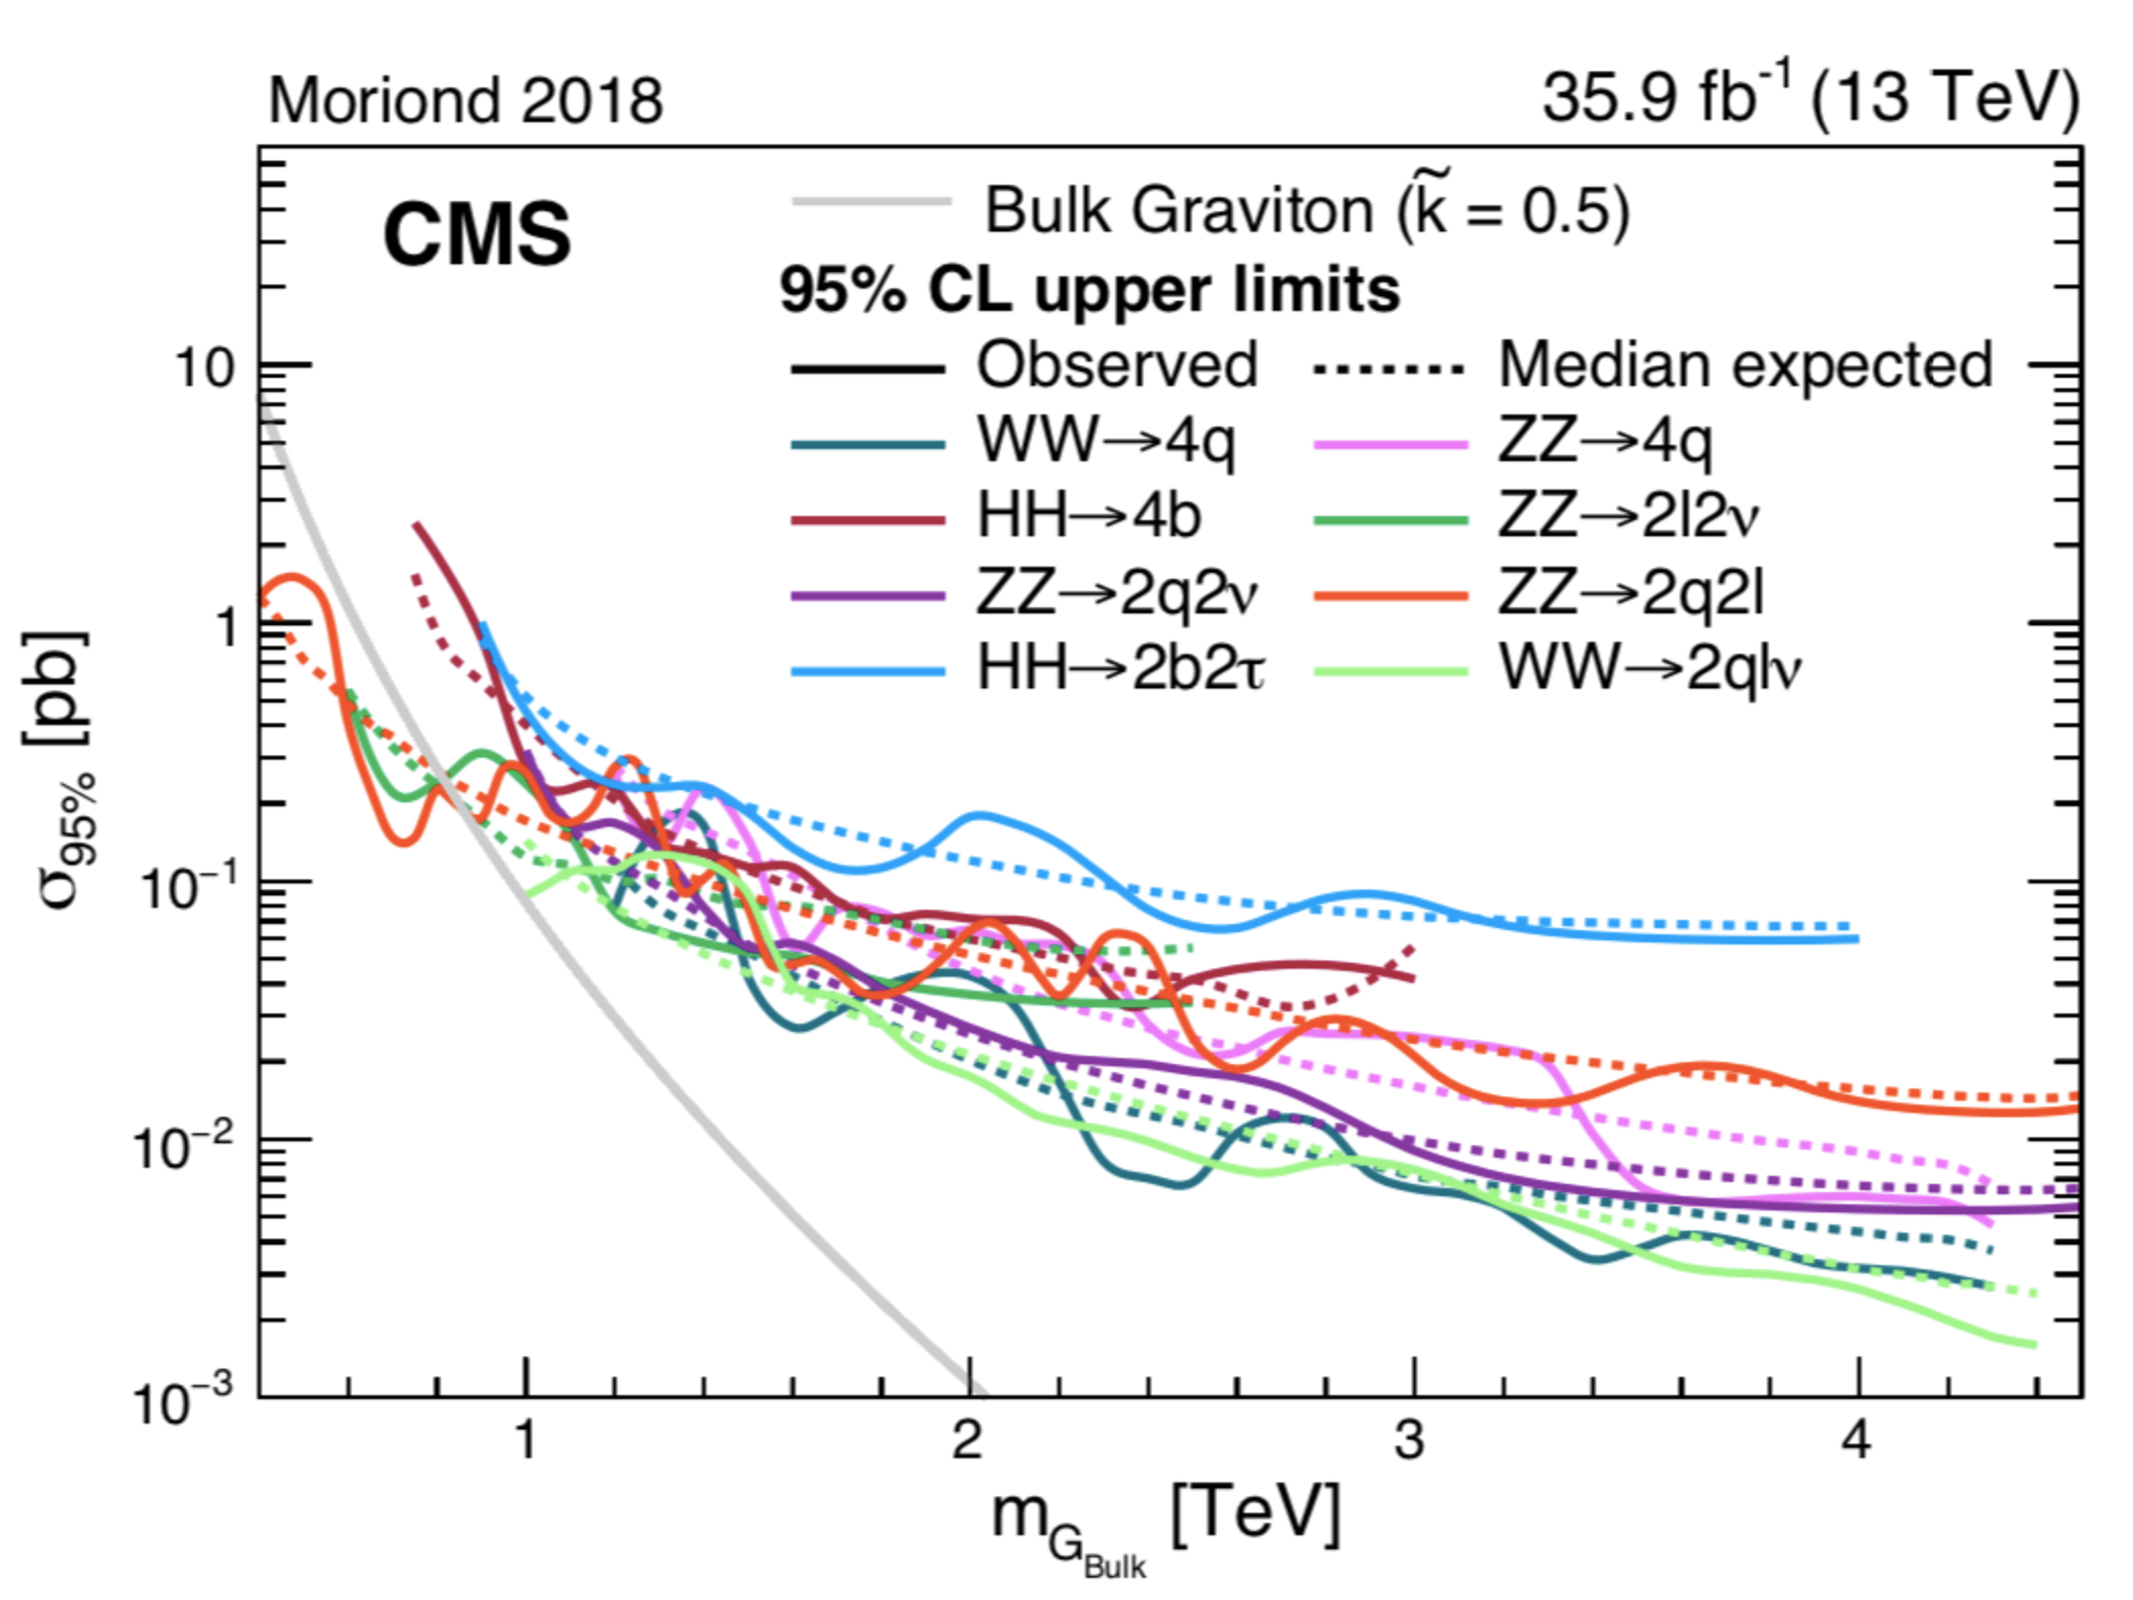
\includegraphics[width=0.9\linewidth]{figures/sum_bulkGlimits.pdf}
\caption{Expected and observed upper limits on the resonance cross section at the 95\% confidence level for various diboson searches based on 2016 CMS full dataset.}
\label{fig:sum_bulkGlimits}
\end{center}
\end{figure}

\vspace{0.3cm}
However the $G_{bulk}\rightarrow ZZ\rightarrow 2\ell 2\nu$ channel suffers low statistics in the highest accessible mass region. With the integrated luminosity of 35.9 fb$^{-1}$, very few events are observed for either signal region data selection or background modeling for $m_T >1000\GeV$. Therefore, this channel is less capable of exploring the region $m_G >2000\GeV$ with the 2016 dataset. Nevertheless, considering that for now statistics is the bottleneck of this analysis, with the 2017 and 2018 CMS data becoming available with data corresponding to an integrated luminosity 3 times as high, a significant improvement in the result is expected from the $G_{bulk}\rightarrow ZZ\rightarrow 2\ell 2\nu$ channel.
